\chapter{How infantry must fight and command within it} 

%\section{Introduction (45 words)}
Rather than rendering mission command obsolete, the Russo--Ukrainian War has reinforced its necessity. Democratised ISR and precision fires expose \gls{c2} to systematic detection and strike --- driving dispersion which prioritises subordinate initiative. As \textcite[208]{busby_2025_military_command_change_21st_century} identifies, mission command's core function is to reduce battlefield uncertainty under such conditions.
What changed was command post survivability. Drones make legacy headquarters systematically vulnerable --- Chornobaivka\index{Chornobaivka HQ} demonstrated tactical echelons could be found and struck \parencite{beagle_slider_arrol_2023_graveyard_command_posts}. Mission command becomes a necessary mitigation as HQs become smaller, dispersed and less visible.

%\section{Digital Visibility, AI and the Fragility of Mission Command (189 words)}

\textcite{METZ_2000} argued that doctrines such as AirLand Battle blended modern technology with mission command and tempo, indicating that technology and decentralisation are not inherently incompatible. Digital systems create persistent incentives toward oversight, even when doctrine prescribes restraint. \posscite{KRULAK_1999} ``strategic corporal'' reflected the link between tactical action and strategic consequence. The legal imperatives of the \gls{GWoT} further institutionalised this dynamic, drawing senior commanders into increasingly granular oversight. As \textcite{BETTS_1996} observes, technology does not improve judgement; it amplifies existing organisational tendencies. Such tendencies are evident among AFRF and AFUA formations, where distant commanders dictate individual soldiers' movements and actions \parencite{dan_participant_1}. ISRDs therefore have an inherent tension simultaneously enabling centralised control and subordinate initiative. Contemporary mission command is thus less a settled doctrine than a contingent practice: the virtual oversight described by \textcite{COHEN_1996} persists, but the dispersion required for survival reinforces the decentralised execution anticipated by \textcite[15]{USMC_MOC_2016}.

%\section{Impact of UxS on Light Infantry Tactics}
Persistent ISR and drone-enabled lethality have forced light infantry to fundamentally rethink tactics, mission command and platoon composition at sub-company level. Battlefield effects are increasingly generated prior to contact --- by machines --- through integrated reconnaissance, strike and counter-reconnaissance systems. Hence, infantry must assume their movements are constantly observed and plan to employ and be engaged by machines, as advised by \textcite[58--63]{fm30}.

While debate persists over the utility of larger drones \parencite{calcara_2022a}, there is little uncertainty regarding the effectiveness of small drone technology's impact on light infantry. Considering Lanchester's force equations --- where Equation~\ref{eq:square} depicts the relative loss rates\footnote{Where \(RLR_i\) is the ratio of attacker to defender loss rates on sector \(i\), $K_{d,i}$ and $K_{a,i}$  are defender and attacker lethality coefficients, and \(F_i=A_i/D_i\) is the local force ratio.} \parencite{davis_1995,lanchester_1916,epstein_1988,hughes_1995a,MEARSHEIMER_1994} --- drones do not make the Russo--Ukrainian War reducible to a pure Lanchesterian duel, in which attrition is treated as mathematically predictable from force strength and lethality coefficients alone. Analysing the lethality coefficients is incomplete, because they are shaped by EW, weather, adaptation and force heterogeneity. Nevertheless, they make local breakthrough combat more Lanchesterian in character by raising the salience of relative lethality and local exposure. Even where both sides possess surveillance and strike drones, the attacker must mass, move, breach and remain observable for longer. The defender by contrast remains comparatively concealed in prepared positions. Battlefield transparency therefore affects attrition asymmetrically. It does not merely improve observation in general. Instead it raises the defender’s effective lethality coefficient $K_{d,i}$  relative to the attacker’s, by increasing the probability of detection, effective engagement and lethality.


\begin{equation}
	RLR_i \equiv \frac{ALR_i}{DLR_i} = \frac{K_{d,i}}{K_{a,i}} \frac{1}{F_i^{2}}
	\label{eq:square}
	%\tag{rlr}
\end{equation}

The central implication follows. Numerical mass becomes a progressively poorer substitute for positional advantage. The result is that the historical 3:1 heuristic likely understates the local superiority now required for successful breakthrough in drone-saturated positional warfare. As \textcite[40:33--44:00]{WATLING_2023_book_launch} notes, drones also narrow the technological gap between peer and sub-peer forces.

Without reliable CUAS (including EW and manoeuvre) UAS become a primary driver of light infantry attrition: directly as OWADs and CASDs or indirectly through ISRD-corrected fires. \textcite[29]{MOLLOY_2024} argues that this is particularly consequential for light infantry operating without reliable access to suppressive fires \parencite[23]{kunertova_2024_2024_08}. UAS contest the immediate airspace above ground forces, as their small size, speed and low-altitude flight profile complicate detection and interception.

%\subection{Light Infantry Offensive Adaptation (594 words)}
The integration of UAS into the battlespace has permanently added a vertical dimension to section-level tactical planning. It requires a task organisation which would have been considered an exceptional measure in pre-drone doctrine\index{Vertical Dimension!Section tactics}. \textcite[17]{watling_2025_10} observes that Ukrainian sections now routinely divide their attention, evenly split between the ground and air --- echoed by \textcite{Liber_Ukraine_1_2026_2_20}. This is not an adaptation to exceptional circumstances. The section commander who plans only for the ground plane now plans for less than half the battlespace.

Within the zone of contestation, advancing on enemy positions becomes prohibitively dangerous unless enemy drones are first suppressed, limiting opportunities for close combat. On quieter sections of the front, small-unit infiltration, raids and ambushes can be effective. The importance of CUAS during offence is underscored by the observation that ``if you don't use anti-drone measures [...] every mission will be a failure'' \parencite{uKR_LESSONS_LEARNED_2}. This places a premium on route planning, dedicated CUAS groups, ER, EW and \textit{hard-kill}\index{Counter UAS!Hard-kill} countermeasures\index{Counter UAS!Electronic reconnaissance}\index{Electronic Warfare}\index{Counter UAS!Electronic Warfare}.


Contemporary Russian tactics illustrate the integration of these dynamics. \textcite[3--4]{watling_2025_10} and \textcite{Zabrodksyi_watling} describe an approach combining reconnaissance, suppressive fires and small-unit infiltration. Forces conduct reconnaissance by fire, build combat power incrementally and exploit degraded enemy ISR and favourable conditions to advance. While effective, this approach exposes light infantry to significant attrition, as evidenced in \textcite{ombr66_2026_03_20_all_arms_Defence}.

For key objectives, dispersion alone is insufficient. Successful offensive action demands fleeting concentration through mobility and kill-chain disruption \parencite[62--63]{ZABRODSKYI_2022}, supported by shaping actions which isolate the enemy via UAS suppression, EW and logistics strikes \parencite{uKR_LESSONS_LEARNED_2,neron_bancel_2024_05_27} and \parencite[ch.~9]{Watling_book}. Deception has regained prominence, understood through the See--Think--Do model, which requires it to induce specific enemy actions (or inaction) rather than mere belief.

\textcite{Stepanenko_2025b} assesses that AFRF FPV-OWADs are likely achieving limited \gls{term:bai}, which raises the threat to \gls{gloc} and logistics. The vulnerability of Russian C2 when deprived of reliable connectivity such as Starlink illustrates this logic. \textcite{Dave_2023_9_1,hallatt_2024_03_13_2,tango_2024_03_13} highlight the dangers of post-assault consolidation, as ISRD-enabled targeting rapidly brings accurate indirect and drone-delivered fires onto newly seized positions. \textcite[5--11]{watling_2025_10} demonstrates that Ukrainian offensive action is no longer conceived as a rapid breach but as a phased contest for local conditions. The sector is first surveyed, then isolated from support and resupply, degraded, fixed and suppressed before assault forces close and consolidate\index{Combined arms}\index{Survey|see{Reconnaissance}}.

Infantry can only close with the enemy as the terminal act of an attritional sequence --- \index{Assault!Culminating act} assault is the exploitation of conditions created by prior shaping phases. Manoeuvre is thus generated not by speed or shock at contact, but by systematically degrading the defender’s capacity to observe, reinforce and respond across the grey zone\index{Contested Zone}. It aligns tempo with the control of the electromagnetic spectrum\index{UAS}. Aggressive \index{Electronic Warfare}\index{Counter UAS!Electronic Warfare}EW during suppression deliberately trades friendly RC UAS utility for enemy paralysis \parencite{watling_2025_10}, thereby heightening an existing premium on indirect fires identified by \textcite{darragh_participant_4,stu_lyle_participant_11}. For Western forces, these lessons underscore that effective \index{Combined Arms!Synchronisation} combined-arms synchronisation under pervasive sensor coverage demands sequencing of effects across space, time and the electromagnetic spectrum --- a \textit{multi-domain operation}. Manoeuvre itself is a conditional phase achieved only once dominance in the middle battle is secured.

%\subection{Light Infantry Defensive Adaptation (115 words)}
Defensively, ISR imposes further constraints. Administration outside of trenches is often impossible, requiring either interconnected trench systems or self-sustaining positions. Robotics offer partial mitigation. \textcite[57]{Watling_book} suggests that such systems can sustain dispersed forces and reduce exposure by enabling resupply without physical movement. While subterranean systems offer protection, they can degrade effective defensive action. Firing ports, though essential for observation and fires, have become liabilities, with FPVDs targeting them directly and rendering even observation hazardous \parencite{neron_bancel_2024_05_27,Tyshchenko_2026_03_20_ukraine_bunker_story}. This indicates the requirement for CUAS barriers and unattended ground sensors to detect humans and electronic reconnaissance\index{Counter UAS!Electronic reconnaissance} to detect RC drones \parencite[59]{ZABRODSKYI_2022}.


%\subection{Counter IED (260 words)}

Armed drones introduce an IED hazard that current light infantry capacity cannot resolve. Improvised munitions are readily adapted for armed drones --- a practice documented on both sides of the Russo--Ukrainian War. In functional terms, armed UAS must be treated as IEDs \parencite{DORD_2022,danny_participant_5}. The improvised nature of firing systems compounds this hazard: \textcite{civdiv_8,dan_participant_1} report that Ukrainian systems generally include safe-arm switches, whereas Russian equivalents often do not. More sophisticated initiators --- including doppler or microwave sensors and concealed switches --- have also been reported, creating \gls{term:voiedied} \parencite{terrogence_2026_1,Terrogence_doppler_radar_initiation_ukraine_2026}. VOIEDs may be indistinguishable from inert or damaged UAS and can be initiated by a wide range of ordinary actions, including passive detection. This renders any enemy drone storage, workshop or launch site a potential IEDD task --- one which cannot safely be cleared by non-specialists.

Successful CUAS does not remove this threat. A downed armed drone requires render-safe at a scale that trained IEDD capacity cannot absorb\footnote{In personal communication with a Bundeswehr IEDD operator (2025), IEDD capacity was assessed as having been reduced by as much as two-thirds following a renewed emphasis on traditional combat engineering; no public source confirming this figure has been identified.}. This forces non-specialists to choose between tolerating the hazard and attempting precarious intervention \parencite[2:58--5:44]{Chosen_9_2024_8_13,garand_thumb_CUAS_2026_3_15} --- necessitating a decentralisation of technical expertise.

Armed drones therefore extend the IED threat vertically \parencite{danny_participant_5}, increasing the burden on small-unit route discipline, clearance drills and hazard awareness. This reinstates the case for a dedicated assault pioneer capability within the battalion support company. It raises the question of whether organic augmentation at section level is warranted \parencite[28:14--30:47]{lyle_23_interview} and \parencite{stu_lyle_participant_11}.


%\subection{Becoming the Least Interesting Target (245 words)}
UAS drive an evolution in the logic of survivability. For the \textcite[6]{USMC_MOC_2016} ``to be detected is to be targeted is to be killed''. Similarly, veterans such as \textcite[9:15--10:55]{Gifford_m_2025325} report that ``the drone will not necessarily kill you, but it will lead to your death if it spots you''. However, evidence from the Russo--Ukrainian War suggests a more nuanced reality, in which the kill-chain may stall after detection. The firer must weigh the value of the target against the cost of ammunition, the expected battlefield effect, competing fire priorities and the risk of revealing their own position and being targeted in return.

Survivability is therefore achieved less through protection or firepower than through becoming the \textit{least interesting target} --- echoed by \textcite[53]{neron_bancel_2024_05_27}. The same logic applies electromagnetically: cheap, low-power commercial radios which hide within civilian noise are harder to detect \parencite{Birchfield_2026}.

For example, robotic CASEVAC may present a less attractive target than a group of stretcher bearers.\footnote{Two interviewees reported being wounded by mortar fire while acting as stretcher bearers; see also \textcite{landforces_ukraine_2026_CASEVAC}.} Similarly, visibly well-equipped formations  attract greater attention than lower-signature troops moving along the same route. Examples include the Russian use of horses instead of vehicles to reduce target value \parencite{Axe_horses_2026}. Interviewees report that foreign legionnaires attracted fire where conscripts on the same routes  did not \parencite{david_participant_2,darragh_participant_4}. Soldiers may even attempt deception, for example by ``playing dead'' \parencite{magyar_telegram_FPV_inf_plying_dead}. Infantry therefore adapt by maximising dispersion, camouflage, timing, unpredictability and signature discipline \parencite{TCAG_Brad}. The survivability onion\index{Survivability Onion} increasingly applies to dismounted infantry and not just vehicles \parencite{Hemez_2017}.


%\subection{Limits of Light Infantry: The Infantry Ceiling (110 words)}


Dispersion preserves infantry survivability but imposes an \textit{infantry ceiling}\index{Infantry Ceiling}: the threshold at which dispersion precludes the concentration of mass required for breakthrough. Where the defender effectively integrates UxS into the kill-chain, the traditional 3:1 offensive heuristic becomes insufficient, as numerical mass increasingly generates targets rather than combat power. Infantry therefore remain essential, but function primarily as survivable fixing elements within a wider system which generates manoeuvre through the sequencing of effects across forces and domains \parencite[5--11]{watling_2025_10}.


%\section{Light Infantry Counter Drone Tactics --- CUAS (477 words)}\index{First Person View One-Way Attack Drone!Light infantry counter tactics}
The UAS threat renders CUAS an enduring light infantry requirement irrespective of operational context. \textcite{stu_lyle_participant_11} argues that the requirement for CUAS at sub-company level is contingent on operational context, increasing in static or positional warfare and diminishing under conditions of manoeuvre. \textcite[vi, 22--23,~31]{hvizda_2025} argue that the drone-enabled stagnation observed in Ukraine is not a permanent feature of  warfare, but a consequence of neither side achieving air superiority. In their account, once NATO gains air control --- assessed as the likely outcome of a NATO--Russia conflict given Western technological overmatch --- persistent UAS-enabled surveillance and strike become less decisive, enabling offensive ground manoeuvre. However, this argument applies only under specific conditions: where air superiority and manoeuvre are achievable. A US--China conflict over Taiwan\index{Taiwan} may differ, producing a maritime and stand-off strike campaign rather than mobile combined-arms ground operations \parencite[34--35]{hvizda_2025}. This is reinforced by \textcite{cancian_2023_first_battle_next_war}, which predicts a positional, attritional defence centred on containing and reducing a beachhead. More fundamentally, even offensive operations are not necessarily characterised by manoeuvre at the tactical level, but by positional, fires-dominated combat \parencite{FOX_2021,KING_2023}. Taiwan therefore shows that the tactical problem is not confined to Ukraine: where an attacker must lodge, move and sustain forces under observation, UxS can turn exposure into a defensive advantage by improving the defender's RCP.

For light infantry --- where UxS lethality is most acutely experienced --- air superiority is tactically remote relative to their immediate exposure. UAS presence is immediate and continuous, requiring adaptation regardless of higher-level operational outcomes. This dynamic is reinforced in operations other than war\index{Counter UAS!Infantry requirement during operations other than war}, where air superiority cannot be assumed, rules of engagement constrain suppression and adversaries can employ UAS at low cost and low political risk \parencite{WATLING_2024} --- entrenching persistent exposure. While equipping units with layered CUAS assets to detect and engage UAS is crucial for force protection, platoon-level CUAS self-defence is inherently constrained. \textcite[28]{WATLING_2024} conclude that the battalion is the smallest unit possible to support organic CUAS.

The underlying issue is contextual. In manoeuvre warfare, the most consequential UAS threat is typically ISRD corrected fires\index{Counter UAS!Requirement during manoeuvre warfare}. Once located, an infantry section is more likely to face suppression by indirect fires than FPVDs. This renders personal CUAS measures of limited operational significance. In this sense, the shotgun solution addresses the terminal symptom while the kill-chain\index{Kill-Chain!CUAS} closes around the shooter. However, the calculus differs in positional warfare, stabilisation/security/peacekeeping tasks and the defence of fixed installations. Here, drones may represent the primary threat and fires-based suppression of UAS teams is neither guaranteed, appropriate nor responsive. The targeting of a US base attributed to Kata'ib Hizbullah\index{Kata'ib Hizbullah!Targeting a US Base} illustrates this dynamic: in such environments, attriting with inexpensive FPVDs becomes feasible precisely because the conditions which render personal CUAS marginal in manoeuvre warfare do not apply. This indicates the value of dispersed, decentralised CUAS effectors, as \textcite[5]{hinote_ryan_2024} advocate.


%\section{Mission Command and Platoon Composition Under Persistent Enemy Surveillance (1539 words)}



%\subsubsection{Dispersed movement and mission command}
Participant interviews and combat footage clearly elucidate the requirement for dispersed, decentralised movement and action. \textcite{darragh_participant_4} is explicit that under drone ISR, sections must fragment into pairs and trios. EW-degraded communications is assumed rather than exceptional\index{Electronic Warfare!Communications degradation}. As he notes, commanders must accept that they ``don't have control'' of their section for extended periods, relying instead on subordinate initiative when plans inevitably fracture under contact \parencite{darragh_participant_4}. 


\textcite[61,196]{fm30} identifies mitigating detection as essential, prescribing multiple axes, extended march intervals and concentration only sufficient to generate favourable force ratios. In Ukraine this manifests as packeted movement, staggered by intervals of $10$--$15$ minutes\index{Packeted movement} --- regrouping in hardened or subterranean rendezvous points. Dispersion does more than complicate centralised control: it precludes it. Hence, every soldier must know routes, timings and actions-on, even requiring privates to function as ``critical thinkers'' \parencite[1:04:00--1:32:00]{murray_tuga}\index{Mission Command!Critical thinkers} --- echoed by \textcite{Leach_curtain,dan_participant_1}. This reflects a broader doctrinal shift toward mission command, comparable to the transition underpinning AirLand Battle, in which initiative at lower echelons became essential to combat effectiveness.  Relinquishing control is psychologically demanding, yet unavoidable \parencite{darragh_participant_4}. \textcite{fred_participant_9} identifies a tension whereby section commanders must occasionally order concentration to achieve tactical effect, thereby exposing troops to heightened drone risk.


Where surprise is unattainable, \textcite{neron_bancel_2024_05_27} argue that only tactical skill and mission command can compensate. This reinforces the value of competent platoon and section leadership, rather than diminishing it. \textcite{TCAG_Brad} --- a foreign advisor to AFUA --- corroborates this directly: centralised control is increasingly impractical, making initiative at section/squad and platoon level a tactical necessity. The implication is significant: pervasive ISR increases the demand for competent infantry leadership.

\textcite[5:20--6:26]{murray_tuga} attribute much of 3rd Assault Brigade\index{Now a Corps sized unit}'s\index{3rd Assault Corps} battlefield performance to its western --- rather than Soviet --- procedures, specifically its empowerment of junior leaders. \textcite[1:04:52--1:32:00]{murray_tuga} describe the rapidly evolving nature of infantry TTPs as necessitating \gls{aar} after each battle --- particularly for junior officers. Even apparently routine factors such as enemy unit rotation can produce markedly different enemy TTPs. Ego was identified as a major barrier to adaptation, while maturity was a key indicator of junior leader effectiveness. \textcite{darragh_participant_4} described how overconfidence preceding a daytime platoon-assault on entrenched positions contributed to severe casualties, illustrating the tactical consequences of leadership hubris.

%\subsubsection{Role of platoon commanders (143 words)}
Platoon commanders retain a decisive role in pre-contact planning, coordination and fires integration. On contact, however, control fragments and execution devolves to dispersed fights\index{Command!Pre-contact orchestration}\index{Control!post-contact degradation} \parencite{darragh_participant_4}. UxS have increased the requirement for coordination, since the battalion is the lowest-echelon at which fires can be meaningfully planned \parencite{WATLING_2025B}. Offensive action is therefore reconstituted as a sequencing problem in which the assault is the culmination of shaping and enabling actions. This dynamic is especially pronounced in urban terrain, where manoeuvre above company level is constrained \parencite{stu_lyle_participant_11} and \parencite[~144--147]{Watling_book}. Hence, decision-making authority --- and the associated cognitive burden --- is concentrated on section and platoon commanders. They must simultaneously prosecute the close fight and serve as information nodes for higher formations. Effective action increasingly depends on the initiative of junior leaders at lance corporal and corporal level.

%adam look at : next generation combat team
%ADP 6-0 - Mission Command: Command and Control of Army Forces


%\subection{Mission Command Enabled by ISR Drones  - (166 words)}
Chapter 1 concludes that ISRDs should be decentralised. While the OODA loop and kill-chain can be dramatically hastened by ISRDs, it can only be realised through communications --- typically verbally or by radio. UAS teams are vulnerable to detection and fires and therefore require protection --- optimised when sited within hardpoints or armoured vehicles. Hence possible advantages offered by ISRDs are vulnerable to the adversary's EW\index{Electronic Warfare!Kill-chain}. 

\posscite{Axe_sound_of_silence_2026} account illustrates that Russia’s drone-enabled, centrally controlled model --- reliant on Starlink, Telegram and even live helmet-camera feeds to higher headquarters --- proved brittle when connectivity collapsed. Ukraine exploited this silence in a manoeuvrist manner --- conditions under which mission command, rather than centralised control, proves most robust.


Reports of poorly trained soldiers having their every battlefield movement dictated over unencrypted radio by a commander observing via UAS are common --- depicted by \textcite{Dogwoof_2000m_Andriivka}. \textcite{dan_participant_1} describes its utility in the real-time correction of gunfire and grenade throwing during a firefight. 


%\subection{Chosen Company Battles at Pervomaisk : A--B Test (268 words)}\index{Pervomaisk!Chosen Company battles at}

\textcite{Chosen_10_24_5_24,Chosen_8_2024_8_13} document two assaults conducted by Chosen Company of the International Legion against the same defensive positions under similar conditions --- supplemented by participant testimony \textcite{dan_participant_1,darragh_participant_4,fred_participant_9,Dave_2024_3_22,hallatt_2024_03_13_1}. The first attack succeeded largely through a manoeuvrist approach. The second --- executed with essentially the same scheme of manoeuvre --- encountered an enemy which had adapted. Following the initial engagement, the defenders integrated ISR drones to correct indirect fires and control UAS strikes. It produced a decisive defensive action. 

The episode illustrates the dynamic described by practitioners: while the attacking unit repeated its earlier plan in part through ``hubris'' \parencite{darragh_participant_4} derived from previous success, the defending force appears to have conducted its own effective AAR and adaptation. The decisive variable was the defender's integration of ISR and strike drones into the kill-chain. The case therefore functions as a natural comparative vignette. It illustrates both how rapidly the drone-enabled battlespace punishes tactical repetition and how leadership ego or failure to adapt can magnify that vulnerability.

As warfare unfolds through continuous cycles of adaptation between adversaries, learning and innovation must occur at every level. This reinforces mission command's demand for decentralised decision-making and rapid bottom-up feedback \parencite{ryan_2022_08_24_adaptation_battle_russia}.


%ADP 6-0 - Mission Command: Command and Control of Army Forces


%\subection{Light Section Composition (452 words)}


Future light-role sections must balance defender/assaulter specialisation, organic ISR/CUAS/UGS integration, habitual versus organic specialists, and scalable command capacity. This thesis synthesises practitioner and expert testimony \parencite{dan_participant_1,darragh_participant_4,fred_participant_9,stu_lyle_participant_11,Watling_book} to propose two analytical constructs. Figure \ref{sec1}'s notional baseline section comprises rifles, a machine gun and a separate commander. Figure \ref{sec2}'s expanded section incorporates ISRD, CUAS and security. \textcite{dan_participant_1} recorded that drone pilots are exceptionally vulnerable when \textit{under glass} (piloting under goggles).

Figure \ref{sec1} presents a notional nine-soldier baseline section: a commander (corporal), two detachment commanders (lance corporals) and two detachments --- one configured around a grenadier and riflemen, the other around a machine gunner, loader and rifleman. The inclusion of lance corporals frees the commander's cognitive bandwidth and preserves simplicity. However, the commander must personally manage all communications and \textit{systems}\index{Systems Operator}, creating a cognitive bottleneck \parencite{stu_lyle_participant_11}. This mirrors the PPC nomenclature, where systems comprise added technology such as battlefield situational awareness. This section remains reliant on higher-echelon CUAS which, during positional tasks, may constitute a \textit{critical vulnerability}. Absent an organic ISRD, all reconnaissance must be performed by dismounted soldiers, exposing them to fire.

Organic capabilities at section level are therefore necessary. A dedicated ISRD/systems operator compresses the kill-chain and protects dismounts, while organic hard-kill CUAS is required to mitigate the latency and critical vulnerability inherent in reliance on battalion-level assets during positional fighting \parencite[28]{WATLING_2024}. Light infantry sections therefore require organic \textit{hard-kill} CUAS to remain tactically viable. Meeting both requirements, while preserving C2 bandwidth and local security, demands additional junior leadership. The downed-drone-as-IED hazard alone justifies an organic assault pioneer --- a requirement compounded by breaching, route proving and hasty fortification under persistent observation.

Accordingly, the smallest viable self-contained section comprises 14 personnel: a commander (corporal), three detachment commanders (lance corporals), two assault detachments of four (each led by a lance corporal and configured as shown in Figure \ref{sec2}) and a  support detachment of five --- integrating ISRD, CUAS, engineer and a rifle --- possibly a sharpshooter with a smart gunsight. This structure retains distinct command and manoeuvre elements, reduces the commander's cognitive burden, facilitates dispersed movement and action, and integrates organic ISR and CUAS at the lowest tactical level.

Mobility imposes a critical constraint across all models. A plausible configuration employs light 4$\times$4 platforms to balance mobility, dispersion and survivability. In the context of light-role reconnaissance, \textcite[~112--113]{Watling_book} suggests a size comparable to a civilian pick-up carrying three soldiers per vehicle (for reserve capacity), reinforcing the need to distribute personnel across multiple platforms. Applying this criterion to six-seat 4$\times$4 platforms, both the nine- and fourteen-soldier models require two vehicles, although multiple vehicles per section introduce non-trivial logistical and coordination burdens \parencite{stu_lyle_participant_11}.

\begin{figure}[H]
	\centering
	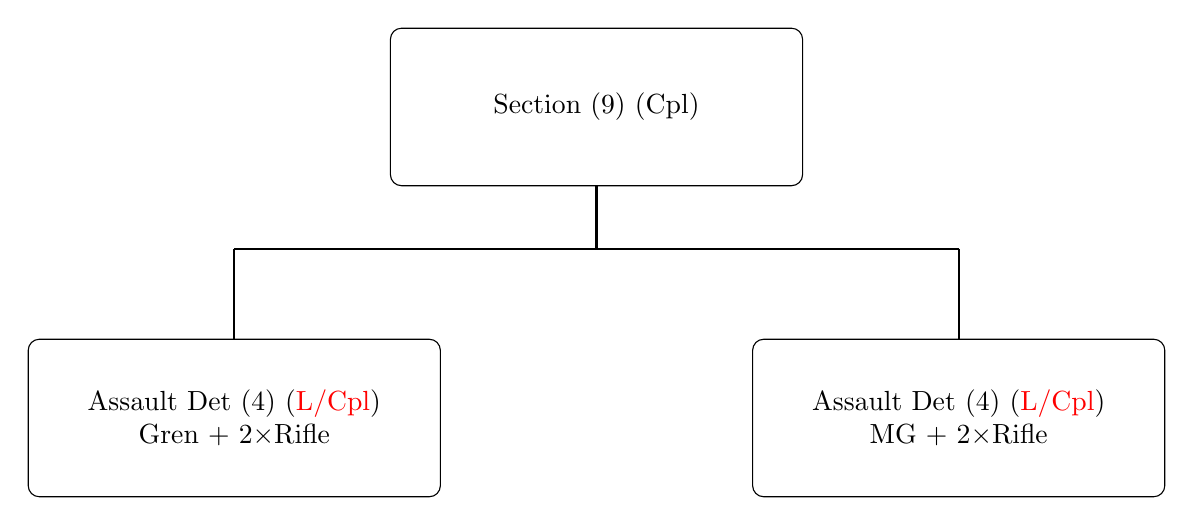
\begin{tikzpicture}[
		box/.style={
			draw,
			rounded corners,
			align=center,
			minimum width=5.2cm,
			minimum height=2cm,
			text width=5cm,
			font=\normalsize,
			fill=white
		},
		line/.style={draw, thick}
		]
		
		% Top node
		\node[box, minimum width=3.8cm] (sec) at (0,0) {Section (9) (Cpl)};
		
		% Left assault det
		\node[box] (ass1) at (-4.6,-3.95) 
		{Assault Det (4) (\textcolor{red}{L/Cpl})\\Gren + 2$\times$Rifle};
		
		% Right assault det
		\node[box] (ass2) at (4.6,-3.95) 
		{Assault Det (4) (\textcolor{red}{L/Cpl})\\MG + 2$\times$Rifle};
		
		
		% Main trunk
		\draw[line] (sec.south) -- (0,-1.8);
		
		% Horizontal branch
		\draw[line] (-4.6,-1.8) -- (4.6,-1.8);
		
		% Branches to assault detachments
		\draw[line] (-4.6,-1.8) -- (ass1.north);
		\draw[line] (4.6,-1.8) -- (ass2.north);
		
		
	\end{tikzpicture}
	\caption[9 Soldier section structure]{Section structure 1: Nine-soldier section with two assault detachments and separate commander}
	\label{sec1}
\end{figure}


\begin{figure}[H]
	\centering
	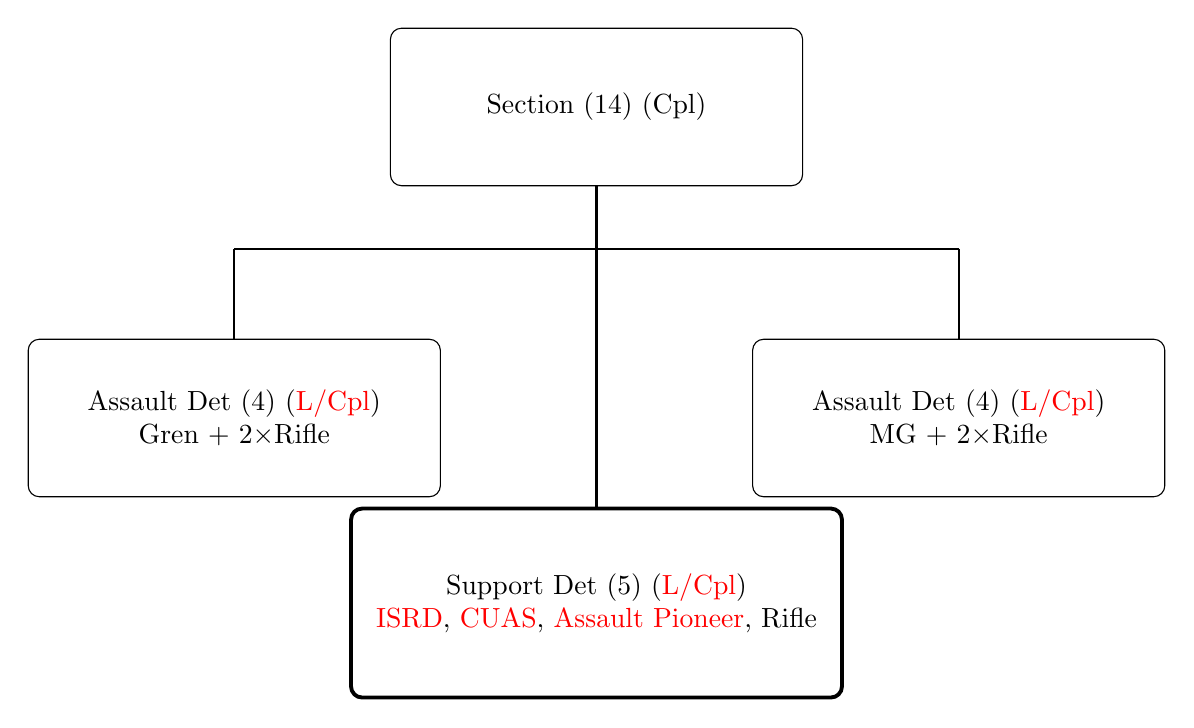
\begin{tikzpicture}[
				box/.style={
			draw,
			rounded corners,
			align=center,
			minimum width=5.2cm,
			minimum height=2cm,
			text width=5cm,
			font=\normalsize,
			fill=white
		},
		supportbox/.style={
			draw,
			rounded corners,
			line width=1.4pt,          % thicker border
			align=center,
			minimum width=6.2cm,       % wider
			minimum height=2.4cm,      % taller
			text width=6cm,
			font=\normalsize,%\bfseries, % bold text
			fill=white                 % no shading
		},
		line/.style={draw, thick}
		]
		
		% Section commander
		\node[box, minimum width=3.8cm] (sec) at (0,0) {Section (14) (Cpl)};
		
		% Assault detachments
		\node[box] (ass1) at (-4.6,-3.95) 
		{Assault Det (4) (\textcolor{red}{L/Cpl})\\Gren + 2$\times$Rifle};
		
		\node[box] (ass2) at (4.6,-3.95) 
		{Assault Det (4) (\textcolor{red}{L/Cpl})\\MG + 2$\times$Rifle};
		
		% Support detachment (larger + thicker + bold)
		\node[supportbox] (sup) at (0,-6.3) 
		{Support Det (5) (\textcolor{red}{L/Cpl})\\\textcolor{red}{ISRD}, \textcolor{red}{CUAS}, \textcolor{red}{Assault Pioneer}, Rifle};
		
		% Structure lines
		\draw[line] (sec.south) -- (0,-1.8);
		\draw[line] (-4.6,-1.8) -- (4.6,-1.8);
		\draw[line] (-4.6,-1.8) -- (ass1.north);
		\draw[line] (4.6,-1.8) -- (ass2.north);
		\draw[line] (0,-1.8) -- (sup.north);
				
	\end{tikzpicture}
	\caption[14 soldier section structure: drone survival minimum]{Section structure 2: Fourteen-soldier section with two assault detachments, support detachment and separate commander --- the drone-survival minimum}
	\label{sec2}
\end{figure}


%\section{Cognitive Fratricide (285 words)}

\textcite[5:50--6:19]{kahn_2024_2_20} and \textcite{darragh_participant_4} describe the significant cognitive burden placed on soldiers in battle. This burden is exacerbated by UAS, which demand simultaneous situational awareness of both the ground and aerial domains. In particular, drones enable ambushes, mines and IEDs to be deployed or repositioned rapidly, rendering previously cleared routes dangerous again. Readiness for contact through scanning arcs in the high-port position may result in tunnelled vision, diverting attention from equally significant threats from above and below.

Tensions arise where the risk of aerial observation in open terrain exceeds the threat posed by ground hazards. In such circumstances, soldiers may prioritise speed of movement, running across exposed ground rather than scanning or proving the absence of mines and IEDs --- with rapid movement perceived as the only viable defence.

The psychological pressure is intensified by the constant auditory signature of drones. The high-pitched buzz alone causes soldiers to take cover instinctively, fostering a pervasive sense that nowhere is safe --- a modern form of \textit{drone shock} comparable to the tank shock of 1939--41 \parencite{MOLLOY_2024,neron_bancel_2024_05_27}. This effect may also serve as a deliberate tool of deception, inducing unnecessary reactive behaviour.

The cognitive burden is not confined to the dismounted soldier. Drone pilots themselves operate under substantial strain \parencite[3:20--5:37]{civdiv_1}. This environment validates \posscite[50]{neron_bancel_2024_05_27} observation that transparency can produce soldiers who see everything, but do not understand. Battlefield transparency imposes its own cognitive penalty. The same volume of sensor data which enables targeting can saturate the capacity to act on it. \textcite{perez} and \posscite[24]{neron_bancel_2024_05_27} concept of ``infobesity''\index{Infobesity} captures how this surplus of information paralyses decision-making at the analytical level. Under these conditions, persistent surveillance does not enhance control; it degrades it, producing \textit{cognitive fratricide}\index{Cognitive Fratricide} and eroding the conditions required for mission command.


%\section{Accelerated Tactical Learning (220 words)}

Combat training feedback loops have compressed dramatically. Practitioner experience now circulates laterally via Discord\index{Discord} and Telegram\index{Telegram}, outpacing official channels by connecting soldiers facing identical tactical problems. ``What is learned in combat this month often reshapes how soldiers train the next month'' \parencite{TCAG_Brad}.

Early UAS employment was ad hoc --- soldiers from non-specialist roles flew drones alongside primary duties. Their battlefield dominance has since driven dedicated units like AFUA's Magyar's Birds\index{Magyar's Birds} and AFRF's Rubicon Centre\index{Rubicon Centre}, exposing institutional lag behind tactical adaptation \parencite{MOLLOY_2024}.

This practitioner-driven dissemination is structural, not exceptional. An analogous pattern was observed within the Irish Army on UNIFIL/UNDOF deployments, where soldiers adopted \textit{Maps.me} when institutional GPS navigation was unavailable. Commercial tools filled critical gaps in speed and accessibility unmatched by defence systems.

Pervomaisk testimony demonstrated that continuous infantry TTP evolution occurs at the lowest tactical level and is enabled by mission command. ISRD and helmet FPV footage --- including adversary material --- enable sport-style ``post-match'' analysis. \textcite{darragh_participant_4} recorded how section-level learning is formalised through structured review processes, reinforcing the rapid adaptation cycle observed in combat. The similar importance of remaining abreast of technological evolution is exemplified by \textcite[1:02:00--1:04:52]{murray_tuga}.

Short, accessible lessons-learned material accelerate this cycle. Section-level influence now shapes enterprise adaptation --- \textcite{mingus_steppe_2026_03_06_hedgerows_kill_webs}: ``soldiers and leaders at the squad level influence the enterprise more than most realize''. 

%\section{Conclusion (128 words)}
Persistence and UxS have fundamentally reshaped light infantry warfare by making exposure, rather than contact, the primary source of risk. Battlefield transparency increases lethality asymmetrically, favouring the prepared defender and forcing dispersion, cognitive overload and rapid adaptation. Mission command is therefore not diminished but necessitated. The 14-soldier light infantry section --- integrating organic ISR, CUAS and additional junior leadership --- emerges as the minimum viable structure for survivable and effective combat in a sensor-saturated battlespace.

These adaptations carry implications beyond the tactical level. A force designed around dispersion, democratised ISR and mission command is not simply more survivable --- it imposes cost differently. How that cost-imposition translates into strategic defensive utility for a small, fiscally constrained state is the subject of Chapter 3.

